\documentclass[11pt]{article}
\def\withcolors{0}
\def\withnotes{0}
%%%%%%%%%%%%%%%%%%%%%%%%%%%%%%%%%%%%%%%%%%%%%%%%%%%%%%%%%%%%%%%%%%%%%%%%%%%%%%%%%%%%
\usepackage[T1]{fontenc}
\usepackage[utf8]{inputenc}

%% Eye-candy
\usepackage{lmodern}
\usepackage{xspace}                                     % Smart spacing with \xspace
\usepackage[protrusion=true,expansion=true]{microtype}  % Improve font rendering

% Striking out text
\usepackage[normalem]{ulem}

%% Math
\usepackage{amsfonts,amsmath,amssymb, amsthm, mathtools}
\usepackage{thm-restate}
\usepackage{dsfont} % For the indicator symbol

% Algorithm environment
\usepackage{algorithmicx,algpseudocode,algorithm}

% Colors (with names)
\usepackage[usenames,dvipsnames,table]{xcolor}

% Quotes: \blockquote command
\usepackage{csquotes}

% Relative sizes for text
\usepackage{relsize}

% Bibliography
%\usepackage[numbers]{natbib}

% Required for the table of results
\usepackage{multirow}
\usepackage{chngpage} % allows for temporary adjustment of side margins

% For the commands such as \capitalisewords
\usepackage{mfirstuc}

% Graphics
\usepackage{tikz}
\usetikzlibrary{arrows}
\usetikzlibrary{calc,decorations.pathmorphing,patterns}

% For indexing
\ifnum\withindex=1
  \usepackage{makeidx}
  \usepackage{ifthen}
  \newcommand\indexed[2][]{\ifthenelse{\equal{#1}{}}{#2\index{#2}}{#2\index{#1}}}
  \makeindex %%%% Enable indexing
\fi
%%\usepackage{showidx} % To debug; does not play well with hyperref

% References and links
\usepackage[backref,colorlinks,citecolor=blue,bookmarks=true]{hyperref}
\usepackage{aliascnt}
\usepackage[numbered]{bookmark}

% Full pages
\usepackage{fullpage}

% Compressed lists
\usepackage[shortlabels]{enumitem}
  \setitemize{noitemsep,topsep=3pt,parsep=2pt,partopsep=2pt} % Uncomment for compact item lists
  \setenumerate{itemsep=1pt,topsep=2pt,parsep=2pt,partopsep=2pt}
  \setdescription{itemsep=1pt}
  
% Package for todo notes.
\ifnum\withnotes=1
  \usepackage[colorinlistoftodos,textsize=scriptsize]{todonotes}
\fi

% For testing and draft: to remove afterwards
\usepackage[english]{babel}
\usepackage{blindtext}

\makeatletter
\@ifundefined{theorem}{%
  % Theorems (each with its own style, all same counter). Cf. http://ftp.math.purdue.edu/mirrors/ctan.org/macros/latex/contrib/hyperref/doc/manual.pdf, p.17
  \theoremstyle{plain} %% Style
  	\newtheorem{theorem}{Theorem}[section]
  	\newaliascnt{coro}{theorem}
  	  \newtheorem{corollary}[coro]{Corollary}
  	\aliascntresetthe{coro}
  	\newaliascnt{lem}{theorem}
  		\newtheorem{lemma}[lem]{Lemma}
  	\aliascntresetthe{lem}
  	\newaliascnt{clm}{theorem}
  		\newtheorem{claim}[clm]{Claim}
	\aliascntresetthe{clm}
	\newaliascnt{fact}{theorem}
 	 	\newtheorem{fact}[theorem]{Fact}
	\aliascntresetthe{fact}
  	\newtheorem*{unnumberedfact}{Fact}
  \newaliascnt{prop}{theorem}
  		\newtheorem{proposition}[prop]{Proposition}
	\aliascntresetthe{prop}
	\newaliascnt{conj}{theorem}
  		\newtheorem{conjecture}[conj]{Conjecture}
	\aliascntresetthe{conj}
  \theoremstyle{remark} %% Style
  	\newtheorem{remark}[theorem]{Remark}
  	\newtheorem{question}[theorem]{Question}
  	\newtheorem*{notation}{Notation}
 	 \newtheorem{example}[theorem]{Example}
  \theoremstyle{definition} %% Style
  	\newaliascnt{defn}{theorem}
 		 \newtheorem{definition}[defn]{Definition}
 	 \aliascntresetthe{defn}
}{}
\makeatother
\providecommand*{\lemautorefname}{Lemma} % For \autoref{} to know the name of lemmas
\providecommand*{\clmautorefname}{Claim}
\providecommand*{\propautorefname}{Proposition}
\providecommand*{\coroautorefname}{Corollary}
\providecommand*{\defnautorefname}{Definition}
\newenvironment{proofof}[1]{\begin{proof}[Proof of {#1}]}{\end{proof}}

%% \email{} command
\providecommand{\email}[1]{\href{mailto:#1}{\nolinkurl{#1}\xspace}}

%% Remarks and notes
\ifnum\withcolors=1
  \newcommand{\new}[1]{{\color{red} {#1}}} % new
  \newcommand{\newer}[1]{{\color{blue} {#1}}} % even newer
  \newcommand{\newest}[1]{{\color{orange} {#1}}} % even even newer
  \newcommand{\newerest}[1]{{\color{blue!10!black!40!green} {#1}}} % you get the idea.
  \newcommand{\ccolor}[1]{{\color{RubineRed}#1}} % Clement
\else
  \newcommand{\new}[1]{{{#1}}}
  \newcommand{\newer}[1]{{{#1}}}
  \newcommand{\newest}[1]{{{#1}}}
  \newcommand{\newerest}[1]{{{#1}}}
  \newcommand{\ccolor}[1]{{#1}}
\fi

\ifnum\withnotes=1
  \newcommand{\cnote}[1]{\par\ccolor{\textbf{C: }\sf #1}} % Clement
  \newcommand{\todonote}[2][]{\todo[size=\scriptsize,color=red!40,#1]{#2}}  
	\newcommand{\questionnote}[2][]{\todo[size=\scriptsize,color=blue!30]{#2}}
	\newcommand{\todonotedone}[2][]{\todo[size=\scriptsize,color=green!40]{$\checkmark$ #2}}
	\newcommand{\todonoteinline}[2][]{\todo[inline,size=\scriptsize,color=orange!40,#1]{#2}}  
  \newcommand{\marginnote}[1]{\todo[color=white,linecolor=black]{{#1}}}
\else
  \newcommand{\cnote}[1]{{{#1}}}
  \newcommand{\todonote}[2][]{\ignore{#2}}
	\newcommand{\questionnote}[2][]{\ignore{#2}}
	\newcommand{\todonotedone}[2][]{\ignore{#2}}
	\newcommand{\todonoteinline}[2][]{\ignore{#2}}
  \newcommand{\marginnote}[1]{\ignore{#1}}
\fi
\newcommand{\ignore}[1]{\leavevmode\unskip} % eat unnecessary spaces before
\newcommand{\cmargin}[1]{\marginnote{\ccolor{#1}}} % Clement

% Shortcuts
\newcommand{\eps}{\ensuremath{\varepsilon}\xspace}
\newcommand{\Algo}{\ensuremath{\mathcal{A}}\xspace} % Algorithm A
\newcommand{\Tester}{\ensuremath{\mathcal{T}}\xspace} % Testing algorithm T
\newcommand{\Learner}{\ensuremath{\mathcal{L}}\xspace} % Learning algorithm L
\newcommand{\property}{\ensuremath{\mathcal{P}}\xspace} % Property P
\newcommand{\class}{\ensuremath{\mathcal{C}}\xspace} % Class C
\newcommand{\eqdef}{\stackrel{\rm def}{=}}
\newcommand{\eqlaw}{\stackrel{\mathcal{L}}{=}}
\newcommand{\accept}{\textsf{ACCEPT}\xspace}
\newcommand{\fail}{\textsf{FAIL}\xspace}
\newcommand{\reject}{\textsf{REJECT}\xspace}
\newcommand{\opt}{{\textsc{opt}}\xspace}
\newcommand{\half}{\frac{1}{2}}
\newcommand{\domain}{\ensuremath{\Omega}\xspace} % Domain of a distribution (default notation)
\newcommand{\distribs}[1]{\Delta\!\left(#1\right)} % Domain of a distribution (default notation)
\newcommand{\yes}{{\sf{}yes}\xspace}
\newcommand{\no}{{\sf{}no}\xspace}
\newcommand{\dyes}{{\cal Y}}
\newcommand{\dno}{{\cal N}}

% Complexity
\newcommand{\littleO}[1]{{o\mleft( #1 \mright)}}
\newcommand{\bigO}[1]{{O\mleft( #1 \mright)}}
\newcommand{\bigTheta}[1]{{\Theta\mleft( #1 \mright)}}
\newcommand{\bigOmega}[1]{{\Omega\mleft( #1 \mright)}}
\newcommand{\tildeO}[1]{\tilde{O}\mleft( #1 \mright)}
\newcommand{\tildeTheta}[1]{\operatorname{\tilde{\Theta}}\mleft( #1 \mright)}
\newcommand{\tildeOmega}[1]{\operatorname{\tilde{\Omega}}\mleft( #1 \mright)}
\providecommand{\poly}{\operatorname*{poly}}

% Influence
\newcommand{\totinf}[1][f]{{\mathbf{Inf}[#1]}}
\newcommand{\infl}[2][f]{{\mathbf{Inf}_{#1}(#2)}}
\newcommand{\infldeg}[3][f]{{\mathbf{Inf}_{#1}^{#2}(#3)}}

% Sets and indicators
\newcommand{\setOfSuchThat}[2]{ \left\{\; #1 \;\colon\; #2\; \right\} } 			% sets such as "{ elems | condition }"
\newcommand{\indicSet}[1]{\mathds{1}_{#1}}                                              % indicator function
\newcommand{\indic}[1]{\indicSet{\left\{#1\right\}}}                                             % indicator function
\newcommand{\disjunion}{\amalg}%\coprod, \dotcup...

% Distance
\newcommand{\dtv}{\operatorname{d_{\rm TV}}}
\newcommand{\totalvardist}[2]{{\dtv\!\left({#1, #2}\right)}}
\newcommand{\hellinger}[2]{{\operatorname{d_{\rm{}H}}\!\left({#1, #2}\right)}}
\newcommand{\kolmogorov}[2]{{\operatorname{d_{\rm{}K}}\!\left({#1, #2}\right)}}
\newcommand{\emd}[2]{{\operatorname{d_{\rm{}EMD}}\!\left({#1, #2}\right)}}
\newcommand{\dist}[2]{{\operatorname{dist}\!\left({#1, #2}\right)}}

% Restriction (functions, sequences, etc.)
\newcommand\restr[2]{{% we make the whole thing an ordinary symbol
  \left.\kern-\nulldelimiterspace % automatically resize the bar with \right
  #1 % the function
  \vphantom{\big|} % pretend it's a little taller at normal size
  \right|_{#2} % this is the delimiter
  }}

% Probability
\newcommand{\proba}{\Pr}
\newcommand{\probaOf}[1]{\proba\!\left[\, #1\, \right]}
\newcommand{\probaCond}[2]{\proba\!\left[\, #1 \;\middle\vert\; #2\, \right]}
\newcommand{\probaDistrOf}[2]{\proba_{#1}\left[\, #2\, \right]}

% Support of a distribution/function
\newcommand{\supp}[1]{\operatorname{supp}\!\left(#1\right)}

% Expectation & variance
\newcommand{\expect}[1]{\mathbb{E}\!\left[#1\right]}
\newcommand{\expectCond}[2]{\mathbb{E}\!\left[\, #1 \;\middle\vert\; #2\, \right]}
\newcommand{\shortexpect}{\mathbb{E}}
\newcommand{\var}{\operatorname{Var}}

% Distributions
\newcommand{\uniform}{\ensuremath{\mathcal{U}}}
\newcommand{\uniformOn}[1]{\ensuremath{\uniform\!\left( #1 \right) }}
\newcommand{\geom}[1]{\ensuremath{\operatorname{Geom}\!\left( #1 \right)}}
\newcommand{\bernoulli}[1]{\ensuremath{\operatorname{Bern}\!\left( #1 \right)}}
\newcommand{\bern}[2]{\ensuremath{\operatorname{Bern}^{#1}\!\left( #2 \right)}}
\newcommand{\binomial}[2]{\ensuremath{\operatorname{Bin}\!\left( #1, #2 \right)}}
\newcommand{\poisson}[1]{\ensuremath{\operatorname{Poisson}\!\left( #1 \right) }}
\newcommand{\gaussian}[2]{\ensuremath{ \mathcal{N}\!\left(#1,#2\right) }}
\newcommand{\gaussianpdf}[2]{\ensuremath{ g_{#1,#2}}}
\newcommand{\betadistr}[2]{\ensuremath{ \operatorname{Beta}\!\left( #1, #2 \right) }}

% Norms
\newcommand{\norm}[1]{\lVert#1{\rVert}}
\newcommand{\normone}[1]{{\norm{#1}}_1}
\newcommand{\normtwo}[1]{{\norm{#1}}_2}
\newcommand{\norminf}[1]{{\norm{#1}}_\infty}
\newcommand{\abs}[1]{\left\lvert #1 \right\rvert}
\newcommand{\dabs}[1]{\lvert #1 \rvert}
\newcommand{\dotprod}[2]{ \left\langle #1,\xspace #2 \right\rangle } 			% <a,b>
\newcommand{\ip}[2]{\dotprod{#1}{#2}} 			% shortcut

\newcommand{\vect}[1]{\mathbf{#1}} 			% shortcut

% Ceiling and floor
\newcommand{\clg}[1]{\left\lceil #1 \right\rceil}
\newcommand{\flr}[1]{\left\lfloor #1 \right\rfloor}

% Common sets
\newcommand{\R}{\ensuremath{\mathbb{R}}\xspace}
\newcommand{\C}{\ensuremath{\mathbb{C}}\xspace}
\newcommand{\Q}{\ensuremath{\mathbb{Q}}\xspace}
\newcommand{\Z}{\ensuremath{\mathbb{Z}}\xspace}
\newcommand{\N}{\ensuremath{\mathbb{N}}\xspace}
\newcommand{\cont}[1]{\ensuremath{\mathcal{C}^{#1}}}

% Oracles and variants
\newcommand{\ICOND}{{\sf INTCOND}\xspace}
\newcommand{\EVAL}{{\sf EVAL}\xspace}
\newcommand{\CDFEVAL}{{\sf CEVAL}\xspace}
\newcommand{\STAT}{{\sf STAT}\xspace}
\newcommand{\SAMP}{{\sf SAMP}\xspace}
\newcommand{\COND}{{\sf COND}\xspace}
\newcommand{\PCOND}{{\sf PAIRCOND}\xspace}
\newcommand{\ORACLE}{{\sf ORACLE}\xspace}

%% Terminology
\newcommand{\pdfsamp}{dual\xspace}
\newcommand{\cdfsamp}{cumulative dual\xspace}
\newcommand{\Pdfsamp}{\expandafter\capitalisewords\expandafter{\pdfsamp}}
\newcommand{\Cdfsamp}{\expandafter\capitalisewords\expandafter{\cdfsamp}}

% L_p norms
\newcommand{\lp}[1][1]{\ell_{#1}}

% Convolution
\DeclareMathOperator{\convolution}{\ast}

%% Terminology
\newcommand{\D}{\ensuremath{D}}
\newcommand{\distrD}{\ensuremath{\mathcal{D}}}
\newcommand{\birge}[2][\D]{\Phi_{#2}(#1)}
\newcommand{\iid}{i.i.d.\xspace}

% Sign
\DeclareMathOperator{\sign}{sgn}

%% Roman numerals
\makeatletter
\newcommand{\rom}[1]{\romannumeral #1}
\newcommand{\Rom}[1]{\expandafter\@slowromancap\romannumeral #1@}
\newcommand{\century}[2][th]{\Rom{#2}\textsuperscript{#1}}
\makeatother

% Hyperref and \autoref{} -- names
\renewcommand{\sectionautorefname}{Section} % To have "Section 5" instead of "section 5" with \autoref{}
\renewcommand{\chapterautorefname}{Chapter} % To have "Chapter 5" instead of "chapter 5" with \autoref{}
\renewcommand{\subsectionautorefname}{Section} % To have "Section 5" instead of "subsection 5" with \autoref{}
\renewcommand{\subsubsectionautorefname}{Section} % To have "Section 5" instead of "subsubsection 5" with \autoref{}
\def\algorithmautorefname{Algorithm}

\newcommand{\ket}[1]{|#1\rangle}
\newcommand{\bra}[1]{\langle #1|}
\def\twobytwomatrix[#1,#2,#3,#4]{
\begin{bmatrix}
	#1 & #2 \\
	#3 & #4
\end{bmatrix}
}

\def\dotproduct[#1,#2]{
\langle #1 | #2 \rangle
}
\newcommand{\transpose}[1]{{#1}^{\rm T}} 			% shortcut
\newcommand{\adjoint}[1]{{#1}^{\dagger}} 			% shortcut

%%%%%%%%%%%%%%%%%%%%%%%%%%%%%%%%%%%%%%%%%%%%%%%%%%%%%%%%%%%%%%%%%%%%%%%%%%%%%%%%%%%%
\usepackage{listings}

\lstset{ %
  backgroundcolor=\color{white},   % choose the background color; you must add \usepackage{color} or \usepackage{xcolor}
  basicstyle=\small,        % the size of the fonts that are used for the code
  breakatwhitespace=false,         % sets if automatic breaks should only happen at whitespace
  breaklines=true,                 % sets automatic line breaking
  captionpos=b,                    % sets the caption-position to bottom
  commentstyle=\color{OliveGreen},    % comment style
  deletekeywords={...},            % if you want to delete keywords from the given language
  escapeinside={\%*}{*)},          % if you want to add LaTeX within your code
  extendedchars=true,              % lets you use non-ASCII characters; for 8-bits encodings only, does not work with UTF-8
  frame=single,                    % adds a frame around the code
  keepspaces=true,                 % keeps spaces in text, useful for keeping indentation of code (possibly needs columns=flexible)
  keywordstyle=\color{blue},       % keyword style
  language=sh,                 % the language of the code
  morekeywords={def,elif,for, from, to, by,while,i, true, false},            % if you want to add more keywords to the set
  numbers=left,                    % where to put the line-numbers; possible values are (none, left, right)
  numbersep=5pt,                   % how far the line-numbers are from the code
  numberstyle=\tiny\color{Gray}, % the style that is used for the line-numbers
  rulecolor=\color{black},         % if not set, the frame-color may be changed on line-breaks within not-black text (e.g. comments (green here))
  showspaces=false,                % show spaces everywhere adding particular underscores; it overrides 'showstringspaces'
  showstringspaces=false,          % underline spaces within strings only
  showtabs=false,                  % show tabs within strings adding particular underscores
  stepnumber=2,                    % the step between two line-numbers. If it's 1, each line will be numbered
  stringstyle=\color{RedViolet},     % string literal style
  tabsize=2,                       % sets default tabsize to 2 spaces
  title=\lstname                   % show the filename of files included with \lstinputlisting; also try caption instead of title
}



% These force using more of the margins that is the default style
\newcommand{\ket}[1]{|#1\rangle}
\newcommand{\bra}[1]{\langle #1|}
\def\twobytwomatrix[#1,#2,#3,#4]{
\begin{bmatrix}
	#1 & #2 \\
	#3 & #4
\end{bmatrix}
}

\def\dotproduct[#1,#2]{
\langle #1 | #2 \rangle
}
\newcommand{\transpose}[1]{{#1}^{\rm T}} 			% shortcut
\newcommand{\adjoint}[1]{{#1}^{\dagger}} 			% shortcut
\newcommand{\QL}{\textsf{QLang}\xspace}

\begin{document}

% Everything after this becomes content
% Replace the text between curly brackets with your own

\title{\QL: Qubit Language}
\author{
  Christopher Campbell
  \and Cl\'ement Canonne
  \and Sankalpa Khadka
  \and Winnie Narang
  \and Jonathan Wong
}
\date{\today}

% You can leave out ''date'' and it will be added automatically for today
% You can change the ''\today'' date to any text you like


\maketitle

% This command causes the title to be created in the document

\section{Introduction}

% An article style is separated into sections and subsections with 
%   markup such as this.  Use \section*{Principles} for unnumbered sections.
In 1965, Gordon Moore predicted that the number of transistors in integrated circuits would double every two years \cite{Moore:65}; up until now, this prediction has been seen to hold with quite an uncanny success. However, due to physical properties of the circuits, the classical architecture of computers cannot sustain such a increase rate.

Amongst the possible ``fixes'' that could allow the race for computational power to go on, a very promising candidate emerged from the last century's advances in Physics; namely, from the field of Quantum Mechanics. Since Richard Feynman suggested in 1982 a new paradigm of computation based on the laws of Quantum physics \cite{Feynman:82}, there has been great progress made in formulating the principles of \emph{quantum computers}, and in studying both their possibilities and limitations (see e.g. \cite{Shor:98,Williams:08,Nielsen:11}). The objective of this project is to design a language that exploits the mathematical foundations and syntax conventions of quantum computing to facilitate the simulation of quantum algorithms.

\subsection{Quantum computing}

In classical computing, data are stored in the form of binary digits or bits. A \emph{bit} is the basic unit of information stored and manipulated in a computer, which in one of two possible distinct states (for instance: two distinct voltages, on and off state of electric switch, two directions of magnetization, etc.). 
The two possible values/states of a system are represented as binary digits, $0$ and $1$.

\subsubsection{Qubit}
In a quantum computer, data are stored in the form of \emph{qubits}, or quantum bits. A quantum system of $n$ qubits is a Hilbert space of dimension $2^n$; fixing any orthonormal basis, any \emph{quantum state} can thus be uniquely written as a linear combination of $2^n$ orthogonal vectors $\{\ket{i}\}_i$ where $i$ is an $n$-bit binary number.

\begin{example}A $3$ qubit system has a canonical basis of 8 orthonormal states denoted 
$\ket{000}$, $\ket{001}$, $\ket{010}$, $\ket{011}$, $\ket{100}$, $\ket{101}$, $\ket{110}$, $\ket{111}$.
\end{example}
\paragraph{Upshot.} A classical bit has only two states, either $0$ or $1$. However a qubit can have  states $\ket{0}$ and $\ket{1}$, or any linear combination of states also known as a \emph{superposition}: %. Hence, a qubit can have an infinitely many states,
\[
	\ket{\phi}=\alpha\ket{0}+\beta\ket{1}
\]
where $\alpha,\beta\in\C$ are any complex numbers such that $\abs{\alpha}^2+\abs{\beta}^2=1$.

\subsubsection{Quantum Gates}
Logical operations, also known as \emph{logical gates}, are the basis of computation in classical computers. Computers are built with circuit that is made up of logical gates. The examples of logical gates are \textsf{AND}, \textsf{OR}, \textsf{NOT}, \textsf{NOR}, \textsf{XOR}, etc. Similarly,  a \emph{quantum gate} is an operation which is a \emph{unitary transformation} on qubits. The quantum gates are represented by matrices, and a gate acts on $n$ qubits is represented by $2^n \times 2^n$ unitary matrix\footnote{That is, a matrix $U\in\C^{2^n\times 2^n}$ such that $\adjoint{U}U=I_{2^n}$, where $\adjoint{\cdot}$ denotes the Hermitian conjugate.}. Analogous to the classical computer which is built from an electrical circuit containing wires and logic gates, quantum computers are built from  quantum circuits containing ``wires'' \ignore{(mostly photons)} and quantum gates to carry out the computation.\medskip

\noindent More on this, as well as the definition of the usual quantum gates; can be found in \autoref{app:quantum:more}.

\subsection {Dirac notation of quantum computation}
In quantum computing, \emph{Dirac notation} is used to represent qubits. Dirac notation provides concise and intuitive representation of complex matrix operations.

More precisely, a column vector $\left[ \begin {array} {c} c_1\\ c_2\\ \vdots\\ c_n \end{array} \right]$ is represented as $\ket{\psi}$, also read as ``ket psi''.  In particular, the computational basis states, also know as \emph{pure states} are represented as $\ket{i}$  where  $i$ is a $n$-bit binary number. For example,
\[
\ket{000}=\begin{bmatrix} 1\\ 0\\ 0\\ 0\\ 0\\ 0\\ 0\\ 0 \end{bmatrix},
\ket{001}=\begin{bmatrix} 0\\ 1\\ 0\\ 0\\ 0\\ 0\\ 0\\ 0 \end{bmatrix},
\ket{010}=\begin{bmatrix} 0\\ 0\\ 1\\ 0\\ 0\\ 0\\ 0\\ 0 \end{bmatrix},
\dots,
\ket{101}=\begin{bmatrix} 0\\ 0\\ 0\\ 0\\ 0\\ 1\\ 0\\ 0 \end{bmatrix},
\ket{110}=\begin{bmatrix} 0\\ 0\\ 0\\ 0\\ 0\\ 0\\ 1\\ 0 \end{bmatrix},
\ket{111}=\begin{bmatrix} 0\\ 0\\ 0\\ 0\\ 0\\ 0\\ 0\\ 1 \end{bmatrix}
\]
Similarly, the row vector $\begin{bmatrix} c^\ast_1 & c^\ast_2  & \dots & c^\ast_n & \end{bmatrix}$, which is also complex conjugate transpose of $\ket{\psi}$, is represented as $\bra{\psi}$, also read as ``bra psi''.\medskip

The inner product of vectors $\ket{\varphi}$ and $\ket{\psi}$ is written $\dotprod{ \varphi }{ \psi }$.
The tensor product of vectors $\ket{\varphi}$ and $\ket{\psi}$ is written $\ket{\varphi} \otimes \ket{\psi}$  and more commonly $\ket{\varphi}\ket{\psi}$.
We list below a few other mathematical notions that are relevant in quantum computing:

\begin{itemize}[-]
\item $z^\ast$ (complex conjugate of elements)\\  if $z=a+ib$, then $z^\ast = a - ib$.
\item $A^\ast$ (complex conjugate of matrices)\\ if $A = \twobytwomatrix[1,6i,3i,2+4i]$ then $A^\ast = \twobytwomatrix[1,-6i,-3i,2-4i]$.
%%%%%%%%%%%%%%%%%%%%%% Transpose of A
\item $\transpose{A}$  (transpose of matrix $A$)\\ if $A = \twobytwomatrix[1,6i,3i,2+4i]$ then $\transpose{A} = \twobytwomatrix[1,3i,6i,2+4i]$.
%%%%%%%%%%%%%%%%%%%%%% Adjoint of A
\item $\adjoint{A}$  (Hermitian conjugate (adjoint) of matrix $A$)\\
Defined as $\adjoint{A} = \left(\transpose{A}\right)^\ast$; if $A = \twobytwomatrix[1,6i,3i,2+4i]$ then $A^{\dag} = \twobytwomatrix[1,-3i,-6i,2-4i]$
%%%%%%%%%%%%%%%%%%%%%% Norm
\item $\norm{\ket{\psi}}$ ($\lp[2]$ norm of vector $\ket{\psi}$)\\
$\norm{\ket{\psi}} = \sqrt{\dotproduct[{\psi}, {\psi}]}$. 
 (This is often used to normalize $\ket{\psi}$ into a unit vector $\frac{\ket{\psi}}{\norm{\ket{\psi}}}$.)
%%%%%%%%%%%%%%%%%%%%%% Other

\item $\bra{\varphi}A\ket{\psi}$ (inner product of $\ket{\varphi}$ and $A\ket{\psi}$). \\
Equivalently\footnote{Recall that we work in a complex Hilbert space: the inner product is a sesquilinear form.}, inner product of $A^{\dag}\ket{\varphi}$ and $\ket{\psi}$

\end{itemize}

\subsection{Quantum Algorithms}
 %A quantum algorithm is a computation process that uses quantum computing to solve a problem.
 \new{A quantum algorithm is an algorithm that, in addition to operations on bits, can apply quantum gates to qubits and measure the outcome, in order to perform a computation or solve a search problem. Inherently, the outcome of such algorithms will be probabilistic.}%for instance, a quantum algorithm is said to \emph{compute a function $f$ on input $x$} if, for all $x$, the value $f(x)$ it outputs is correct with high probability.
  The representation of a quantum computation process requires an input register, output register and unitary transformation that takes a computational basis states into linear combination of computational basis states. If $x$ represents an $n$ qubit input register and $y$ represents an $m$ qubit output register, then the effect of a unitary transformation $U_f$ on the computational basis $\ket{x}_n\ket{y}_m$ is represented as follows:
	\begin{equation}
	U_f(\ket{x}_n\ket{y}_m)=\ket{x}_n\ket{y\oplus f(x)}_m,
	\end{equation}
	where $f$ is a function that takes an $n$ qubit input register and returns an $m$ qubit output and $\oplus$ represents mod-$2$ bitwise addition.
 \subsubsection{Deutsch-Jozsa Algorithm}
 Deutsch's Problem is an example of a quantum algorithm that performs computation in fewer steps than a classical computer.\\
 Suppose \new{$f\colon\{0,1\}^n \to \{0,1\}$ and that $f$ is either constant or balanced.}  The goal is determine which one it is.  Classically it is trivial to see that this would require (in worst case) querying just over half the solution space, or $2^{n-1} + 1$ queries.  The Deutsch-Jozsa algorithm answers this question with just {\it one} query!
 
\begin{figure}
\begin{center}
  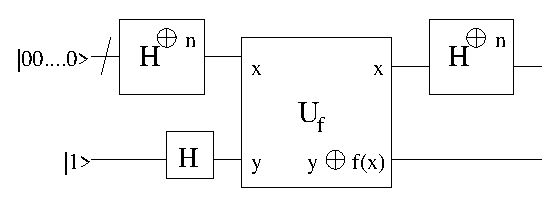
\includegraphics{deutschjozsa}
\end{center}
\caption{Quantum Circuit for Deutsch-Jozsa Algorithm\label{m42}}
\end{figure}

\section {Qubit Language}
	
	The objective of \QL language is to allow simulation of quantum algorithm.
		
\subsection{Syntax}

An operation, or language elementary unit, starts from the end of the previous one, and ends whenever a semicolon or a line return is encountered. In particular, a semicolon at the end of the line is valid, yet not necessary.

\subsubsection{Comments}
Comments will be preceded by symbol \#; after the symbol, the remainder of the line is considered as a comment. No multiline comment is supported.
\begin{lstlisting}[frame=single]
	# This is just a comment.
\end{lstlisting}
	
\subsubsection {Variable Declaration}
Variables are declared with the name of the variable followed by equals and value assigned to the variable.

\begin{lstlisting}[frame=single]
	a = 5.9  
	b = 4+5i
	c = |00>
\end{lstlisting}

A variable name must start with a lower case letter, and can only contain \texttt{ASCII} characters: \texttt{a-aA-Z}, \texttt{0-9}, \_: that is, it must match the pattern \texttt{[a-z][a-zA-Z0-9\_]*}.

\subsubsection{Reserved keywords}
The following words are reserved, and cannot be variable \new{names: \texttt{i}, \texttt{if}, \texttt{elif}, \texttt{else}, \texttt{def}, \texttt{while}, \texttt{for}, \texttt{from}, \texttt{to}, \texttt{by}, \texttt{true}, \texttt{false}, as well as the identifiers of the builtin constructs of \autoref{ssec:operations}.}

\subsubsection{Data Types}

\begin{itemize}
\item Complex numbers\\
Quantum computation is done over complex vector space and hence one of the main data types  is complex number.

\begin{lstlisting}[frame=single]
	a = 5.9  
	b = 4+5i
\end{lstlisting}
All numbers are complex; the keyword \texttt{i} is reserved and refers to the usual value (imaginary unit $i$). By default, all numbers are internally stored as real numbers. \new{The implementation takes care of precision issues in a transparent fashion: the syntax does not differentiate between different floating-point precisions, and the programmer can implicitly assume all numbers have ``infinite precision''.} 

The two particular keywords \texttt{true} and \texttt{false} are constants, equal to respectively $1$ and $0$, and provided for notational convenience. Although we refer to them as Booleans, they are internally considered are complex numbers and can be used as such.

%\cnote{How do we want the precision to be handled? I'd love to have an exact, formal representation with no float/double loss; i.e., a formal representation. By default, integers or finite precision: whenever needed, the internal data type switches to the right representation, eg $\pi$ is representation formally as $\pi$, etc).}

\item Qubits \\
Qubit representation follows Dirac notation.\\

\begin{lstlisting}[frame=single]
	a=|1000>
	b =<001|
	c= |100> + | 110> 	 
\end{lstlisting}

\item Vector and Matrices \\
In essence, all data type are matrices.\\

\begin{lstlisting}[frame=single]
	a=[ 1, 1, 3]
	a=[ 1, 2, 3 ; 4, 5, 6; 7, 8, 9]
\end{lstlisting}

\end{itemize}

\subsubsection{Operations}\label{ssec:operations}
Mathematical operations such as multiplication, division, addition, tensor product matrix multiplication are supported by the language.
\begin{lstlisting}[frame=single]
	a = 5*5
 	b = 5*(6+7i)
	c = H|00>
  	d = |00> @ |1>
	M = [ 1, 2, 3 ; 4, 5, 6; 7, 8, 9]
	N = [1, 2; 5, 6]
	D = M @ N
\end{lstlisting}
Other builtin constructs are $\texttt{transp}$, $\texttt{adj}$, $\texttt{isunit}$, $\texttt{det}$ (for matrices), $\texttt{norm}$, $\texttt{conj}$ (for complex numbers). Note that no support by default is provided for matrix inversion; this choice is due to the fact that most matrices considered will (and have to) be unitary, in which case getting the inverse is straightforward which the above.

\subsubsection{Control Flow}

\begin{lstlisting}[frame=single]
	# if-elif-else statement
	if ( variable == true){
	}elif (boolean){
	}else{
	}
	#for loop, increment by 2 (the `by 2'' is optional
	for k from 1 to 10 by 2 {
	}
\end{lstlisting}
		
\subsubsection{Functions}

\begin{lstlisting}[frame=single]
	def output = function_name(args){
	}
\end{lstlisting}
	
\subsection{Simulation of Deutsch-Jozsa Algorithms} 

\begin{figure}
\begin{center}
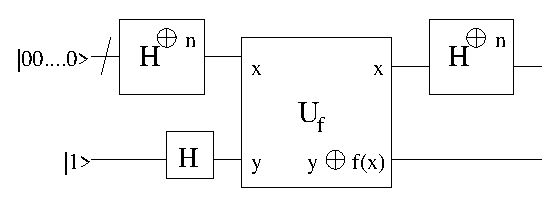
\includegraphics{deutschjozsa}
\end{center}
\caption{ Quantum Circuit for Deutsch-Jozsa Algorithm
\label{m42}}
\end{figure}

\begin{lstlisting}[frame=single]
	def outcome = deutschjozsa(in-qubit, U-matrix){
		
		input-registers = in-qubit @ |1>;
		after-Hadamard = (H @ H)*(input-registers);
		after-U = U-matrix * after-Hadamard;
		after-Had = (H @ I)*after-U;
		M0=((in-qubit*(in-qubit)^H) @ I)*after-Had;
		
		if (M0 == 0){
			outcome = 0;
		}
		else{
			outcome = 1;
		}
	
	}
\end{lstlisting}
\newpage
\section* {The Team}

\begin{description}

\item[Manager:] Jonathan Wong
\item[Language Guru:] Sankalpa Khadka
\item[System Architect:] Winnie Narang
\item[System Integrator:] Cl\'ement Canonne
\item[Verification and Validation:] Christopher Campbell.
\end{description}
These roles are not definitive: each member of the team will work on every aspect of the project, while being the main responsible for its particular area.

\newpage
\nocite{*}
\bibliographystyle{alpha}
\bibliography{references}
\newpage
\appendix
\section{More on quantum computing and the underlying mathematics}\label{app:quantum:more}

\subsection {Common quantum gates}

\subsubsection*{Pauli Operators}
	The \emph{Pauli operators} are the special single qubit gates which are represented by the Pauli matrices $\{I, X, Y, Z\}$ as follows
	\[
I =
\begin{bmatrix}
 1 & 0  \\
 0 & 1  
\end{bmatrix}
\qquad
X =
\begin{bmatrix}
 0 & 1  \\
 1 & 0  
\end{bmatrix}
\qquad
Z =
\begin{bmatrix}
 1 & 0  \\
 0 & -1  
\end{bmatrix}
\qquad
Y =
\begin{bmatrix}
 0 & -i  \\
 i & 0  
\end{bmatrix}.
\]
For example, the application of $X$ causes bit-flip in following ways:
\[
X\ket{0}=\begin{bmatrix}
 0 & 1  \\
 1 & 0  
\end{bmatrix}
\begin{bmatrix}
 1   \\
 0   
\end{bmatrix}=\begin{bmatrix}
 0   \\
 1   
\end{bmatrix}= \ket{1}
\]
\[
X\ket{1}=\begin{bmatrix}
 0 & 1  \\
 1 & 0  
\end{bmatrix}
\begin{bmatrix}
 0   \\
 1   
\end{bmatrix}=\begin{bmatrix}
 1   \\
 0   
\end{bmatrix}= \ket{0}.
\]
\subsubsection*{Hadamard Gate}
The \emph{Hadamard gate} is defined by the matrix:
\[
H= \frac{1}{\sqrt{2}}\begin{bmatrix}
 1 & 1  \\
 1 & -1
\end{bmatrix}.
\]
The Hadamard gate maps the computational basis states into superposition of states. The Hadamard gate is significant since it produces maximally entangled states from basis states in the following ways:
\[
H\ket{0}=\frac{1}{\sqrt{2}}(\ket{0}+\ket{1})
\qquad
H\ket{1}=\frac{1}{\sqrt{2}}(\ket{0}-\ket{1}).
\]

\subsubsection*{Controlled-U Gates}
	A \emph{controlled-U gate} is the quantum gate in which the $U$ operator acts on the \new{$n$\textsuperscript{th} $n$-qubit} only if the value of the preceeding qubit is $1$.\\ For example: In a Controlled-\textsf{NOT} gate, the \textsf{NOT} operator flips the second qubit if the first qubit is $1$.
	\[
	\textsf{CNOT} = \begin{bmatrix}
 1&0&0&0\\
0&1&0&0\\
0&0&0&1 \\
0&0&1&0\end{bmatrix}
	\]
	
	\[
	\textsf{CNOT}\ket{00}=\ket{00}
	\]
	\[
	\textsf{CNOT}\ket{01}=\ket{01}
	\]
	\[
	\textsf{CNOT}\ket{10}=\ket{11}
	\]
	\[
	\textsf{CNOT}\ket{11}=\ket{10}.
	\]
	
	
\subsection {Tensor product and its properties}

Let $A=(a_{i,j})$ be a matrix with respect to the ordered basis $\mathcal{A}=(u_1,\dots,u_n)$ and $B=(b_{i,j})$ be a matrix with respect to the ordered basis $\mathcal{B}=(v_1,\dots,v_m)$. Consider the ordered basis $\mathcal{C}=(u_i \otimes v_j)$ ordered by lexicographic order, that is $u_i \otimes v_j \leq u_l \otimes v_k$ if if $i<l$ or $i=l$ and $j<k$. The matrix of $A \otimes B$ with respect to $\mathcal{C}$ is : 
\[
	A \otimes B= 
	\begin{bmatrix}
 	a_{1,1}B & a_{1,2}B & \dots & a_{1,n}B\\
	a_{2,1}B & a_{2,2}B & \dots & a_{2,n}B\\
	\vdots & \vdots & \ddots & \vdots \\
	a_{n,1}B & a_{n,2}B & \dots & a_{n,n}B
	\end{bmatrix} 
\]
		This matrix is called the tensor product of the matrix $A$ with the matrix $B$.
\begin{itemize}
\item $A \otimes B \otimes C =  (A \otimes B ) \otimes C = A \otimes (B \otimes C)$
\item $ a ( \ket{x} \otimes \ket{y}) = a \ket{x} \otimes \ket{y} = \ket{x} \otimes a\ket{y}$
\item $ ( A \otimes B) \cdot (\ket{y}\ket{z}) = A\ket{y} \otimes B\ket{z}$
\item $ ( A \otimes B) \cdot ( C \otimes D) = AC \otimes BD$
\item $ (A \otimes B) ^{H} = A^{H} \otimes B^{H}$
\item If $ A$ and $B$ unitary, $A \otimes B$ is unitary.
\item If $\ket{x}=\ket{x_1} \ket{x_2}$ and $\ket{y}=\ket{y_1}\ket{y_2}$ then $\dotproduct[x,y]=\dotproduct[x_1,y_1] \dotproduct[x_2, y_2]$ 
\end{itemize}
	
\end{document}
